In this report, the main project choices and the results for structural ensemble PED00020 of measles virus nucleoprotein (for its five deposited ensembles) are reported.

\section{Task 1}\label{sec:task1}
\graphicspath{ {./figures/} }

The goal of the first task is to implement a tool to identify conformational relationships thanks to models structural features within an ensemble. The input is a set of files, each containing the PDB structure of one ensemble, which will be analyzed independently.

\subsection{Single conformation features}

For each conformation, the following structural features are extracted and subsequently saved:
\begin{itemize}
\item[-] \emph{Radius of gyration} (RG) is computed from the coordinates of each atom and their barycenter.
\item[-] \emph{Relative accessible surface area} (ASA) is computed for each residue thanks to DSSP\footnote{\textbf{DSSP}: the values obtained for the conformations within an ensemble are equal. It may happen that the DSSP does not return the ASA value for some residues: for this limitation, a check on the array dimension and, if needed, a zero-padding are performed. }.
\item[-] \emph{Secondary structure} (SS) is determined for each residue thanks to the Ramachandran regions\footnote{\textbf{SS}: for the first and last residue, for which the value is not computable, `-' is inserted.} associated to Phi and Psi angles. For an easiest subsequent analysis, each value is converted into an integer as reported in table \ref{tab:ss}.
\item[-] \emph{Distance matrix} contains the pairwise distances between each pair of residues. For an easiest analysis, since it is symmetric, only the linearized version of its upper triangular sub-matrix is considered.
\end{itemize}

\begin{table}[H]
\begin{center}
\begin{tabular}{lc}
% FIRST ROW
\textbf{Secondary Structure} & \textbf{Int}\\
\hline
- & 0\\
\hline
Beta-sheet & 1\\
\hline
Polyproline I-II & 2\\
\hline
Alpha-helix & 3\\
\hline
Left-handed Helix & 4\\
\end{tabular}
\end{center}
\caption{Conversion for Secondary Structure values}~\label{tab:ss}
\end{table}


\subsection{Representative conformations}
In order to extract the representative conformations, the models are clustered due to \emph{K-Medoids} approach and a customized metric function, selecting the optimal number of clusters thanks to Silhouette score.
\emph{K-Medoids} has been chosen since at the end the representative conformations will be medoids selected between the input set points, without generating unseen conformations.

\medskip
The implemented metric\footnote{\textbf{Metric}: take in input feature vectors of two conformations and compute their distance as sum of partial features distances.} is tailored for each feature set, in order to measure the dissimilarity between models. The following distance metrics have been chosen according to the meaning and the behaviour of single features:
\begin{itemize}
\item[-] Absolute difference between radius of gyration to understand its variation.
\item[-] Euclidean distance of ASA vectors.
\item[-] Normalized hamming distance between SS vectors using the scoring matrix reported in table \ref{tab:score} and defined accordingly to their definition and properties.

\begin{table}[H]
\begin{center}
\begin{tabular}{c|ccccc}
% FIRST ROW
& 0 & 1 & 2 & 3 & 4 \\
\hline
0 & 0 & 1 & 1 & 1 & 1\\
1 & 1 & 0 & 1 & 1 & 1\\
2 & 1 & 1 & 0 & 1 & 1\\
3 & 1 & 1 & 1 & 0 & 0.5\\
4 & 1 & 1 & 1 & 0.5 & 0\\
\end{tabular}
\end{center}
\caption{Scoring matrix Secondary Structure values}~\label{tab:score}
\end{table}

\item[-] Cosine distance between distance matrix.
\end{itemize}

In table \ref{tab:silhouette} we report both the optimal number of clusters and the corresponding silhouette scores obtained with the described clustering procedure for the analyzed ensembles.

\begin{table}[H]
\begin{center}
\begin{tabular}{ccc}
% FIRST ROW
\textbf{Ensemble} & \textbf{Cluster} & \textbf{Silhouette}\\
\hline
001 & 4 & 0.538269\\
\hline
002 & 3 & 0.511878\\
\hline
003 & 4 & 0.499020\\
\hline
004 & 3 & 0.521289\\
\hline
005 & 3 & 0.545507\\
\end{tabular}
\end{center}
\caption{Silhouette values obtained during clustering}~\label{tab:silhouette}
\end{table}

Afterwards, a weighted graph is built, inside which each node is a representative model with edge length between pairs of nodes proportional to the distance between correspondent pairs of conformations according to the built metric. In figures \ref{model001}, \ref{model002}, \ref{model003}, \ref{model004} and \ref{model005}, built graphs are reported.

\begin{figure}[H]
    \centering
	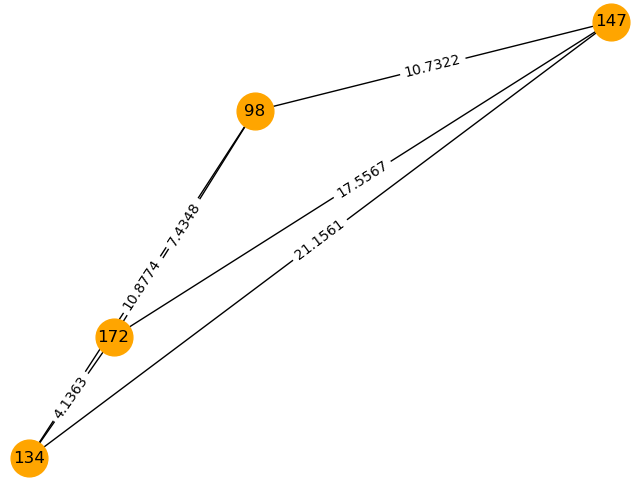
\includegraphics[width=\textwidth]{PED00020e001_graph.png}
	\caption{Graph of ensemble 001.}
	\label{model001}
\end{figure}

\begin{figure}[H]
    \centering
		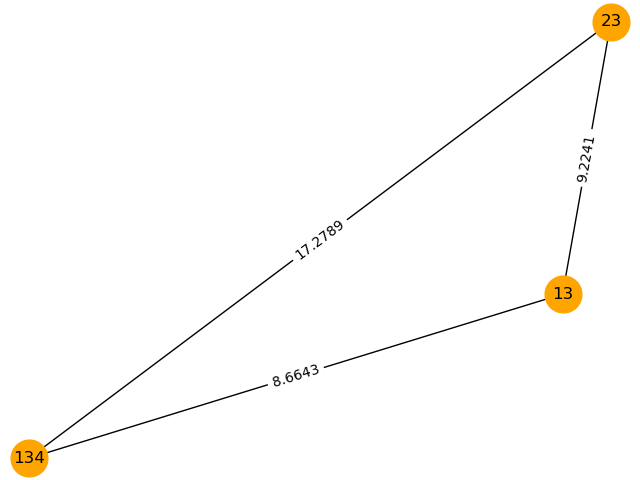
\includegraphics[width=\textwidth]{PED00020e002_graph.png}
		\caption{Graph of ensemble 002.}
		\label{model002}
\end{figure}

\begin{figure}[H]
    \centering
		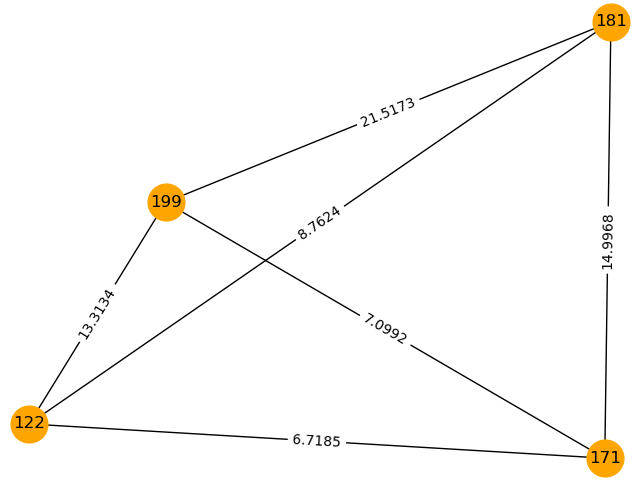
\includegraphics[width=\textwidth]{PED00020e003_graph.png}
		\caption{Graph of ensemble 003.}
		\label{model003}
\end{figure}

\begin{figure}[H]
    \centering
		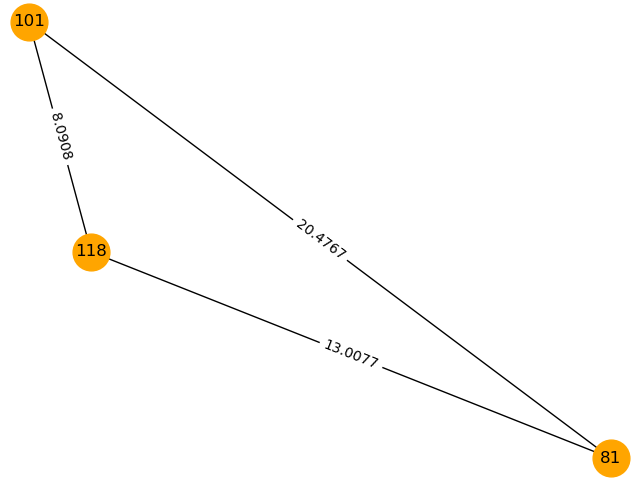
\includegraphics[width=\textwidth]{PED00020e004_graph.png}
		\caption{Graph of ensemble 004.}
		\label{model004}
\end{figure}

\begin{figure}[H]
    \centering
		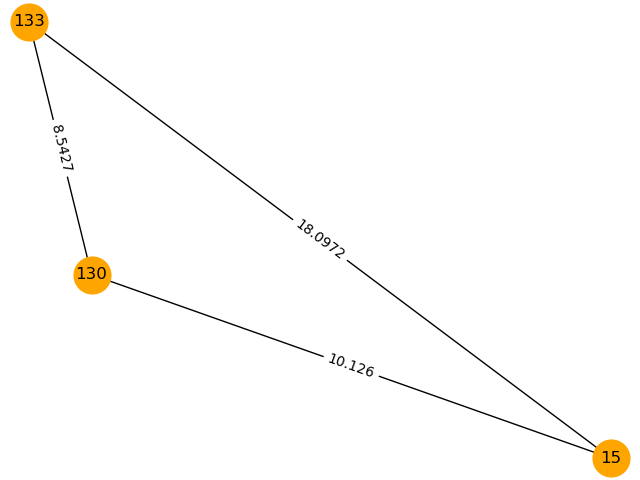
\includegraphics[width=\textwidth]{PED00020e005_graph.png}
		\caption{Graph of ensemble 005.}
		\label{model005}
\end{figure}

A high results variability can be observed, in terms of selected medoids but not in the optimal number of clusters.
This is probably caused by two main factors:
\begin{itemize}
    \item[-] Proximity of the points in the features space.
    \item[-] Random initialization of medoids during clustering.
\end{itemize}

\subsection{Pymol image}
A Pymol image is generated to visualize the 3D structure of one representative conformation and the variability of each residue.
We decided to generate one image for each ensemble, instead of the superimposition of all the conformations, because latter would give a too messy result without any important information.
In order to reduce the computing time needed to compare the features\footnote{\textbf{Pymol}: the time needed for the Pymol image generation considering the features over all the models is about one hour.}, we have decided to take into consideration only features of representative conformations, since each one of them is a good approximation of its own cluster.

\medskip
The i-th residue variability is calculated using a customized metric, which considers a window of 19 (9 before and 9 after) residues around the current one. After extracting the features vectors of those residues for each considered conformation, the metric calculates the variability as the sum of the following partial distances:
\begin{itemize}
\item[-] Standard deviations of ASA values for each residue are calculated and their mean is computed to obtain an average window value.
\item[-] Normalized hamming distances between SS vectors pairs are calculated using the scoring matrix reported in table \ref{tab:ss}.
\item[-] Cosine dissimilarities are computed and summed for each pair of analyzed conformations between distance vectors of corresponding residues.
\end{itemize}
Note that the radius of gyration is not used since it is not residue-dependent.

\medskip
A BWR color-map\footnote{\textbf{BWR} : is a color-map that use blue, white and red color to characterize respectively low, mid and high values inside a plot.} is used to highlight which residues own the highest or lowest variability inside each Pymol image.
Looking at figures \ref{model001p}, \ref{model002p}, \ref{model003p}, \ref{model004p} and \ref{model005p}, it is possible to notice that structures are in general very disordered since contains few well-defined secondary structures, that in these cases are only alpha-helices. This may happen because the entropic high cost of folding. %%???
Further considerations about the protein structure are provided in the conclusions of this report.

\begin{figure}[H]
    \centering
		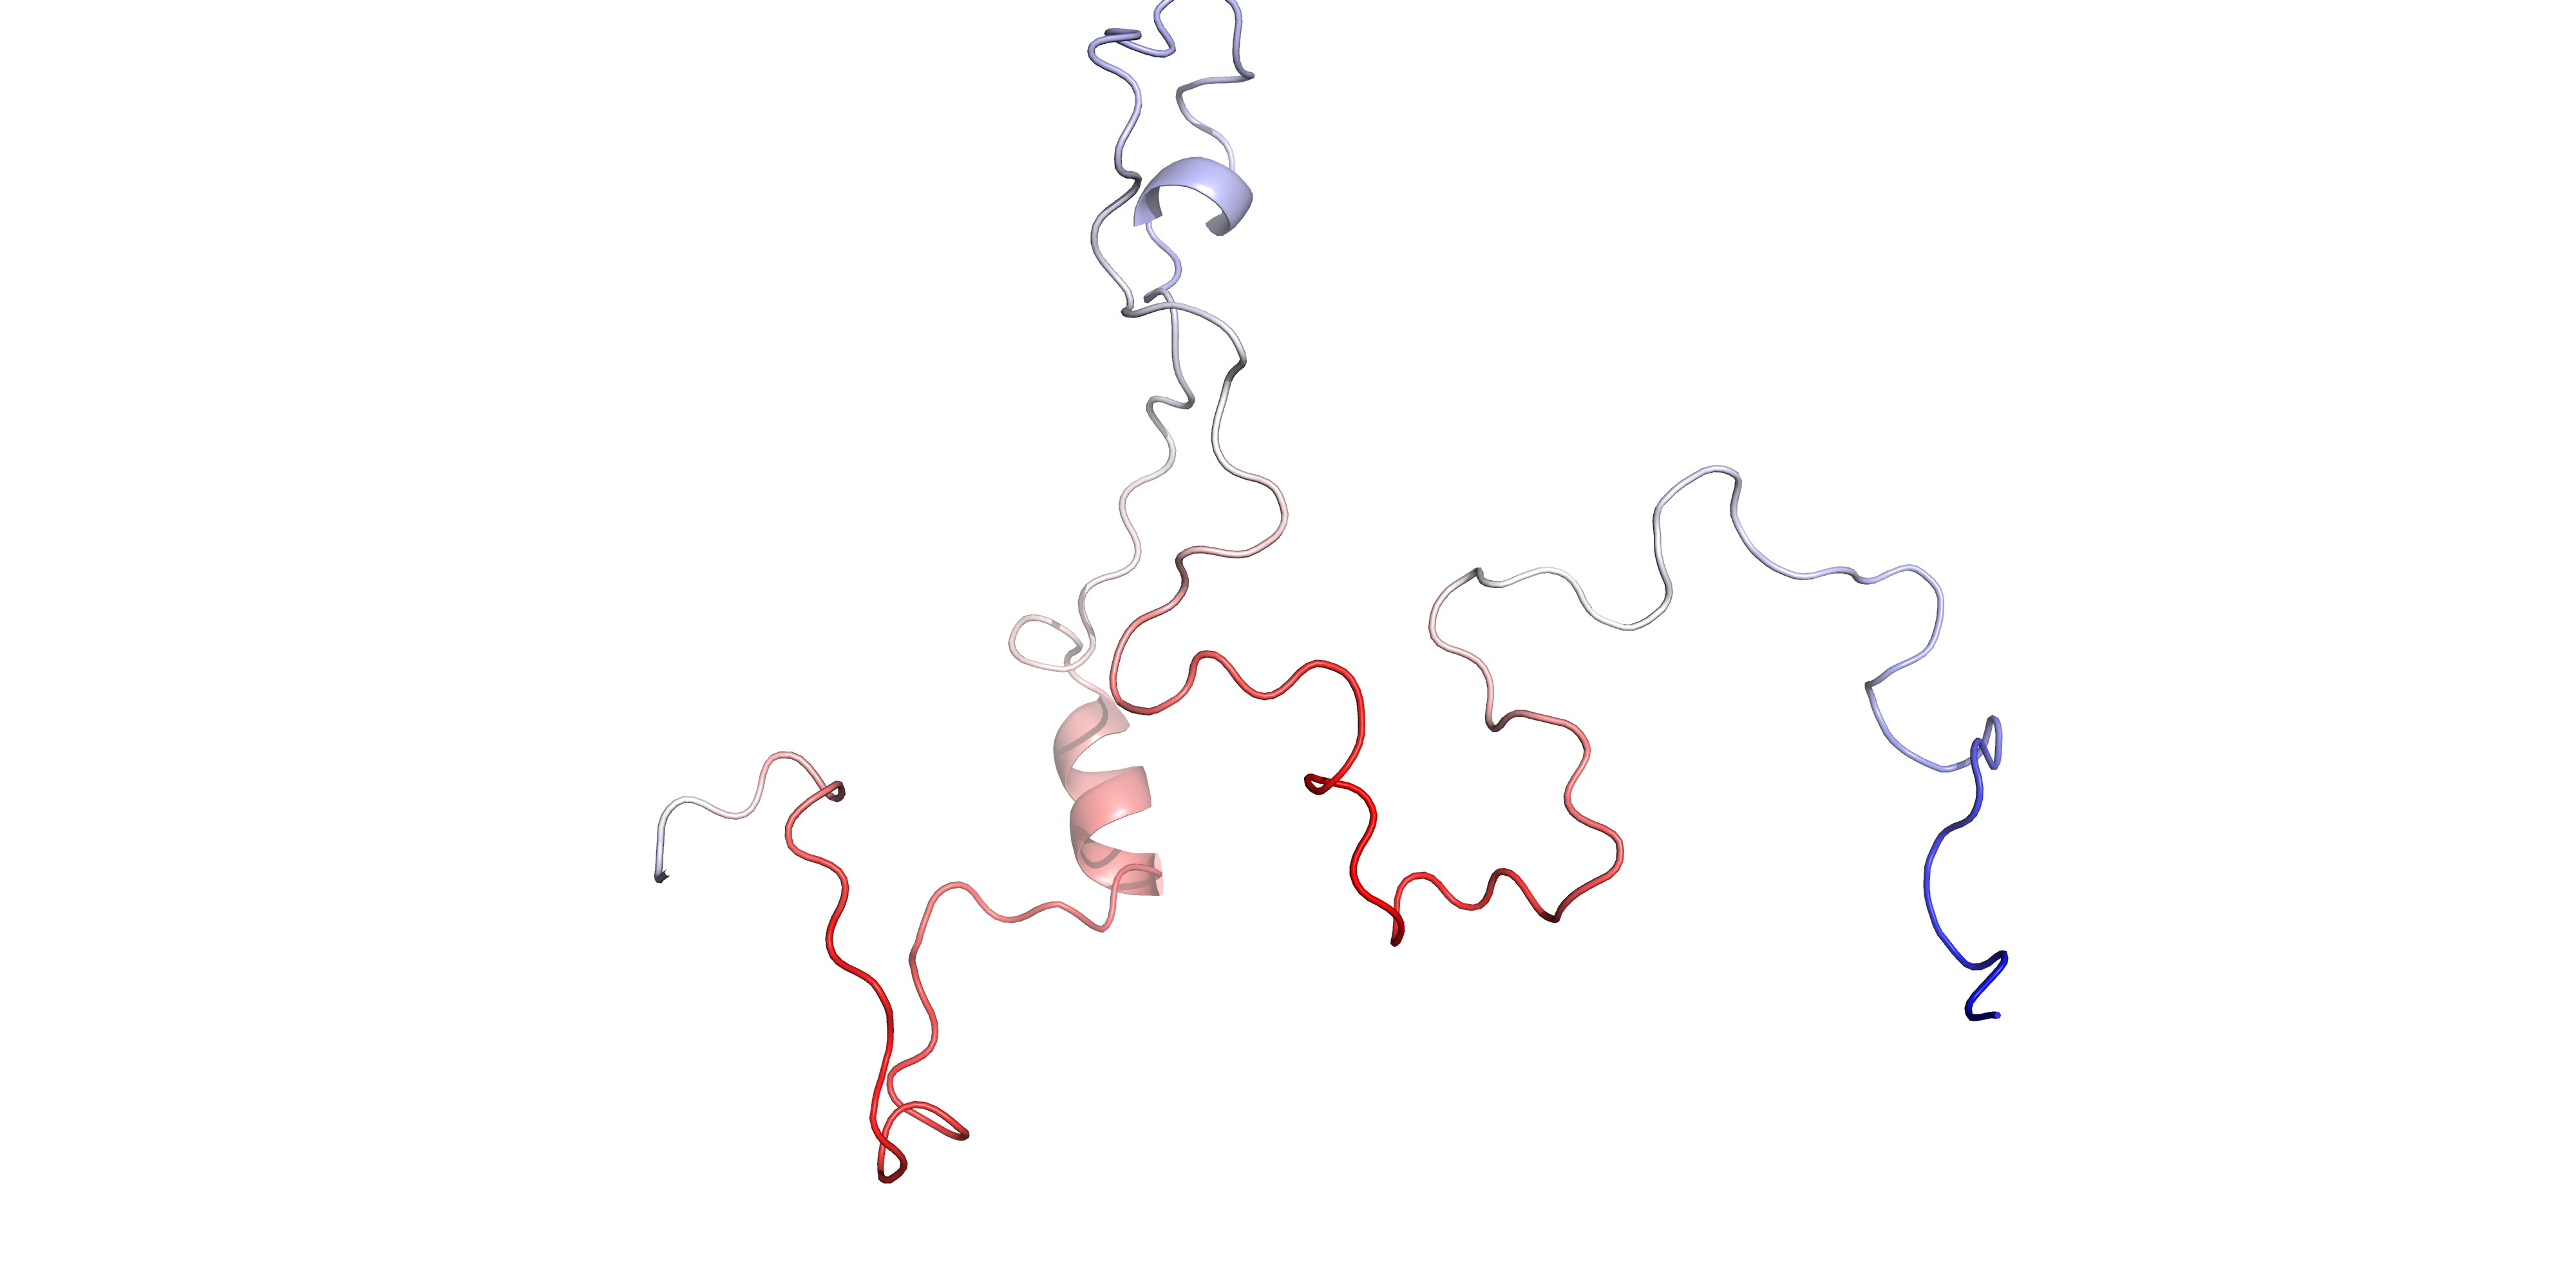
\includegraphics[width=\textwidth]{PED00020e001_pymol.png}
		\caption{Pymol image of ensemble 001 (model 098).}
		\label{model001p}
\end{figure}

\begin{figure}[H]
    \centering
		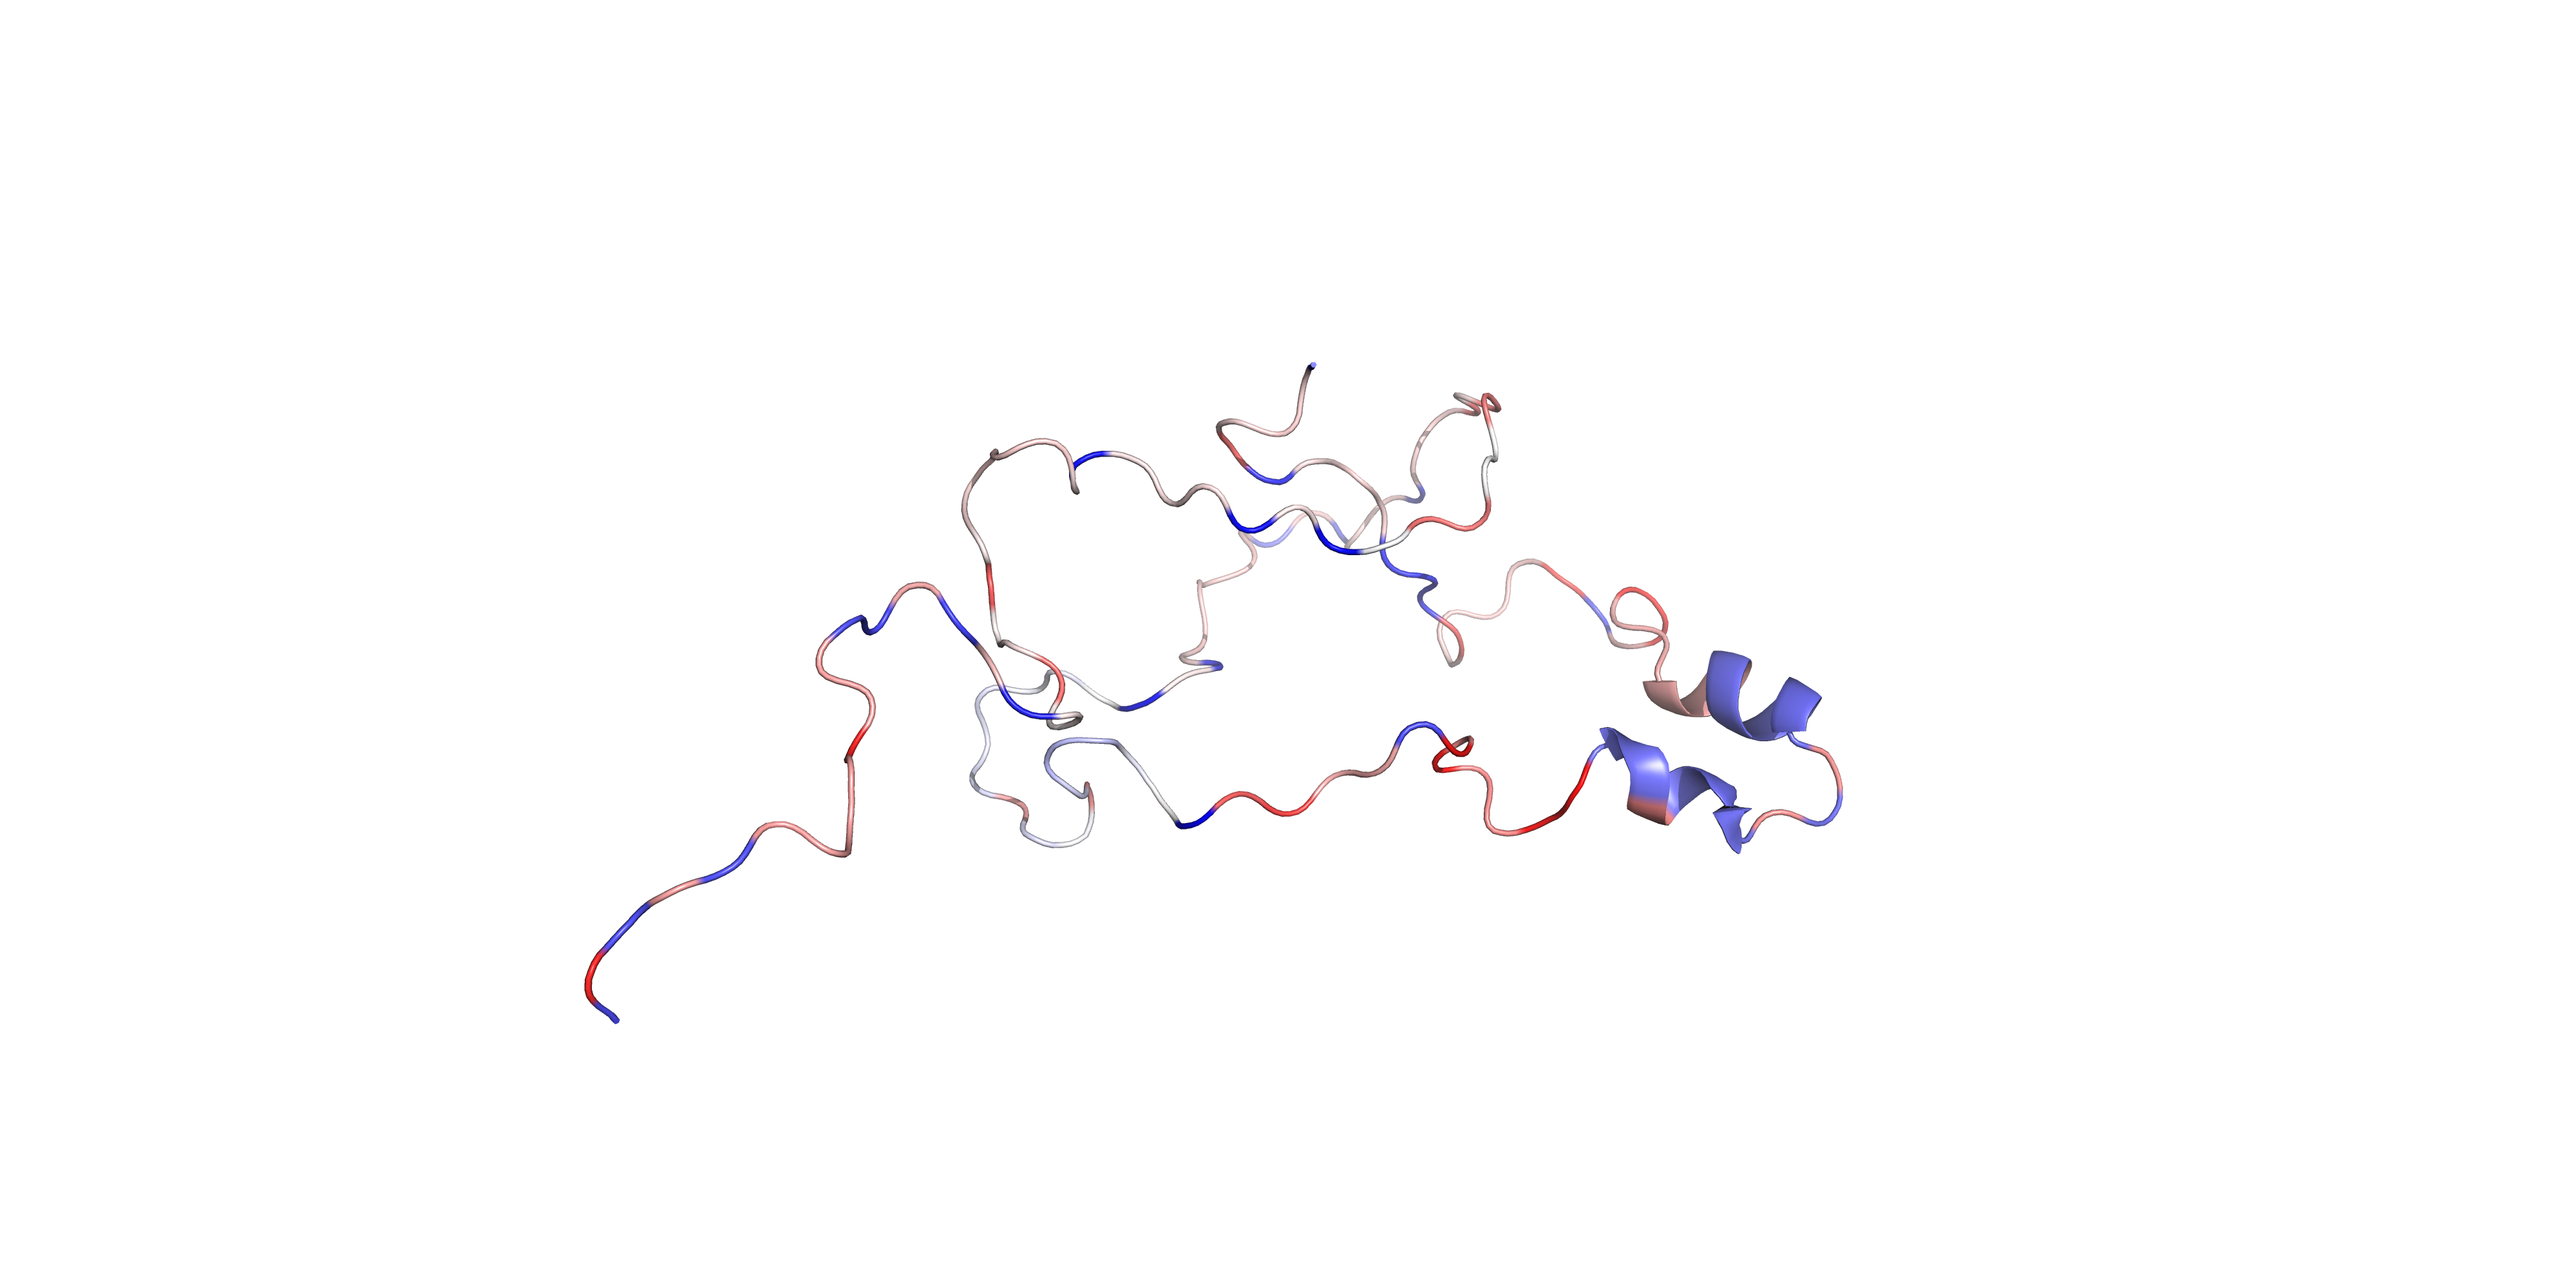
\includegraphics[width=\textwidth]{PED00020e002_pymol.png}
		\caption{Pymol image of ensemble 002 (model 023).}
		\label{model002p}
\end{figure}

\begin{figure}[H]
    \centering
		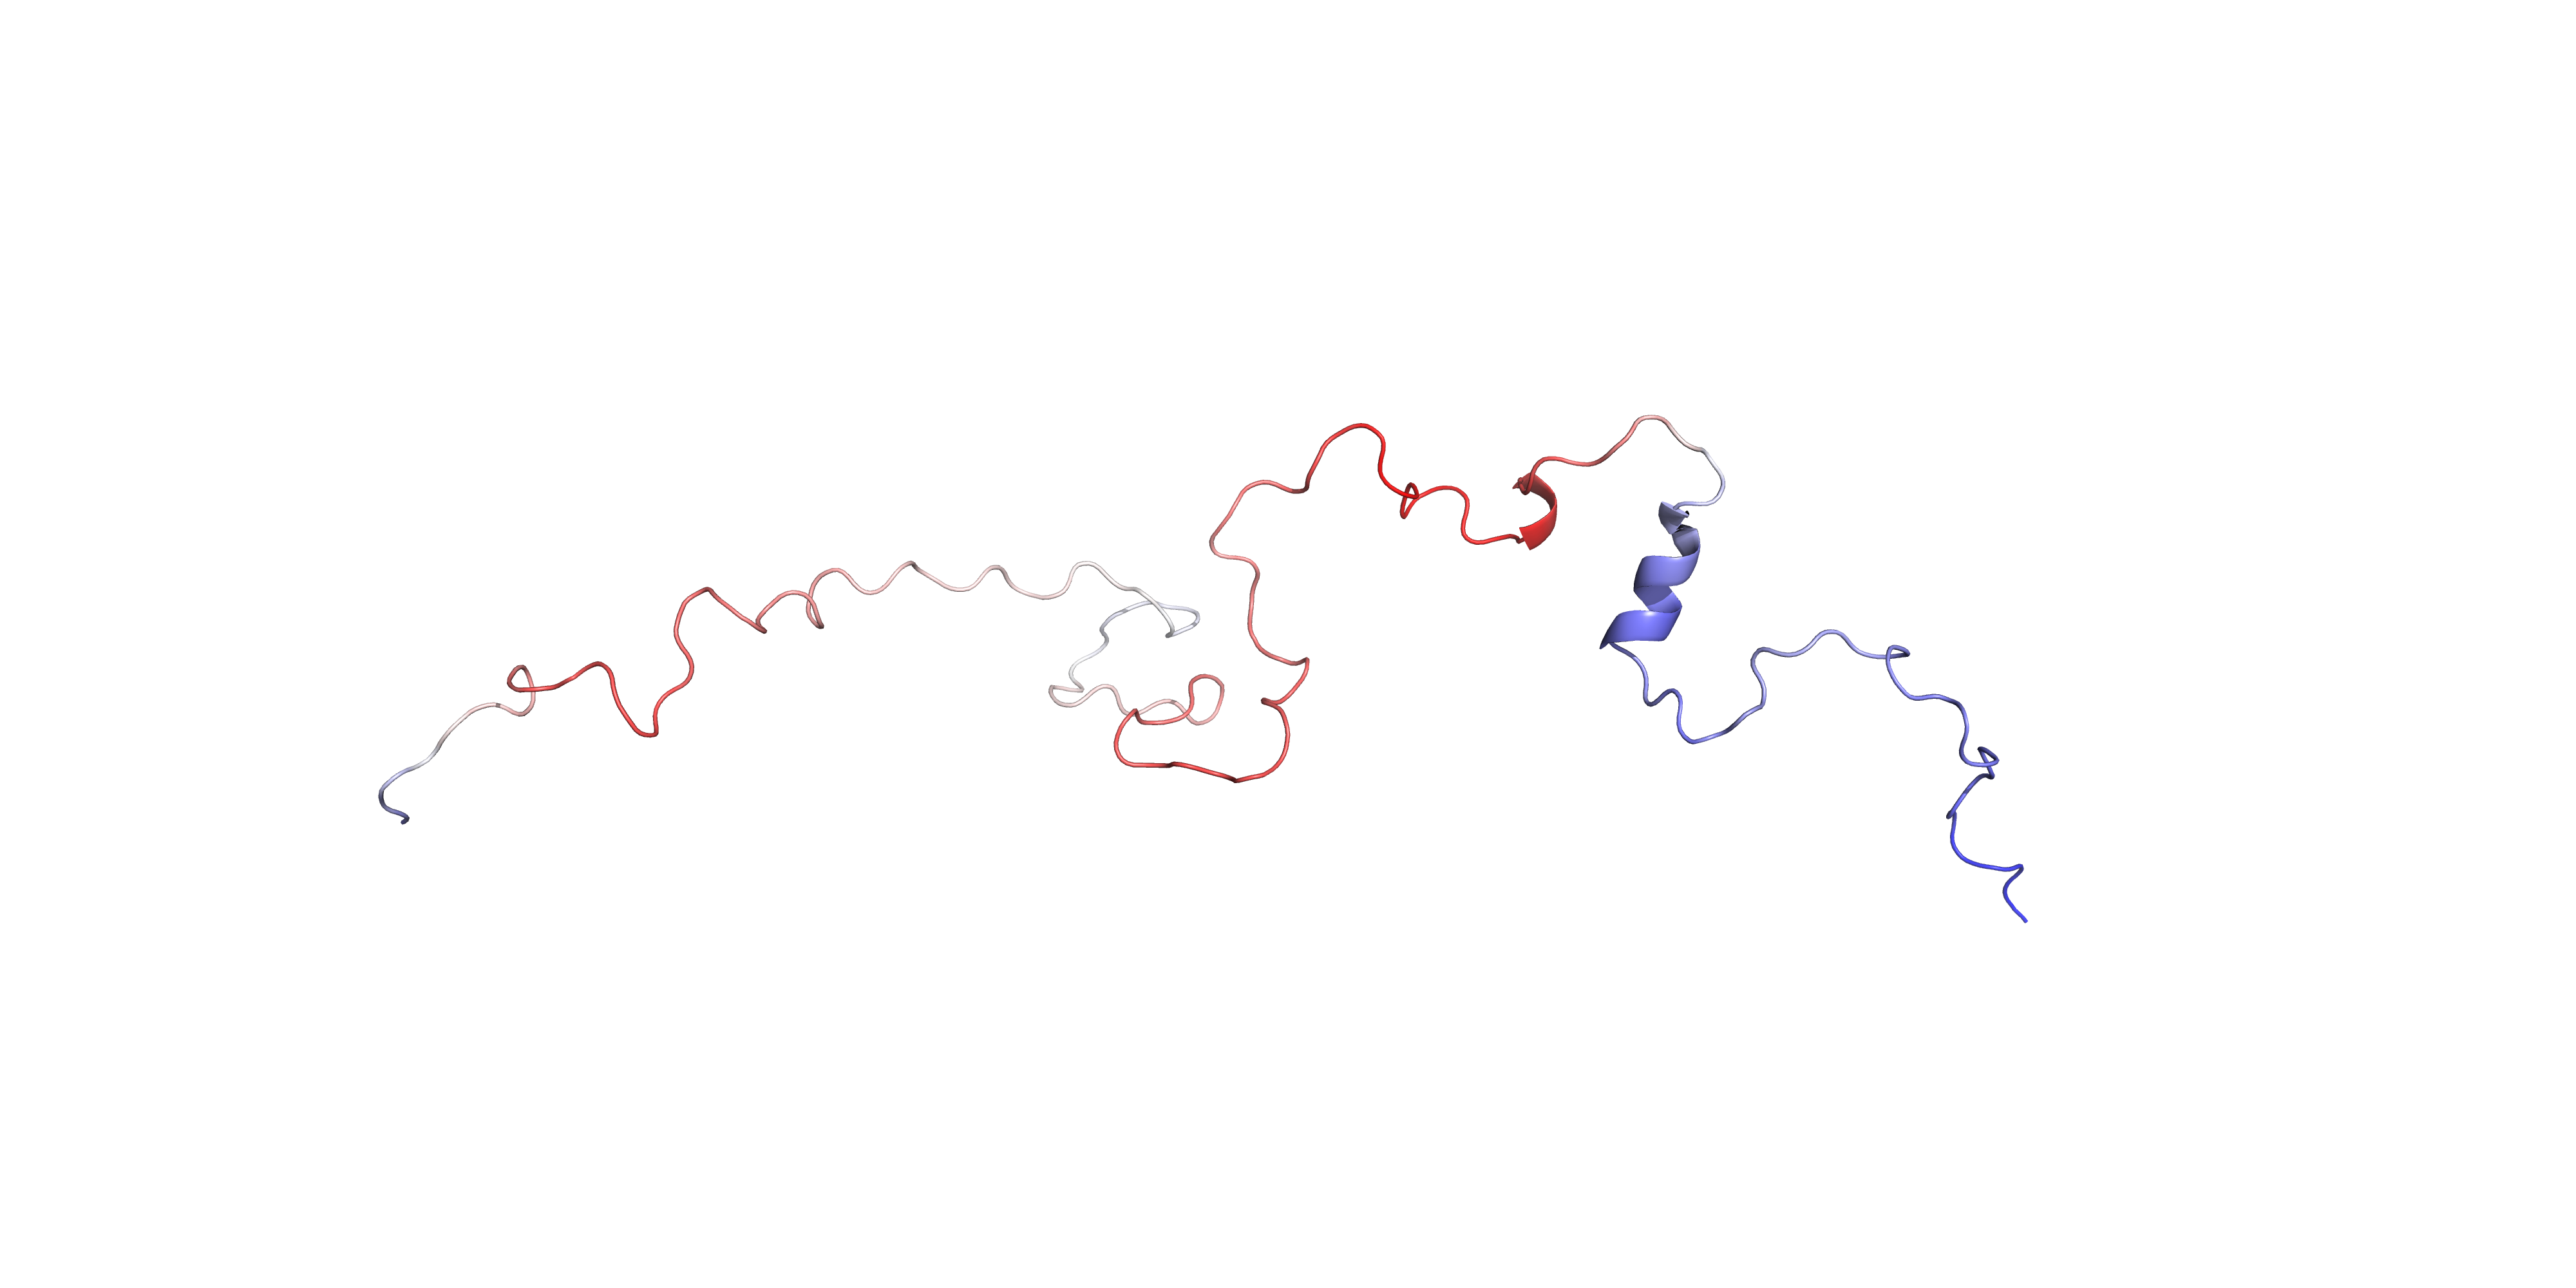
\includegraphics[width=\textwidth]{PED00020e003_pymol.png}
		\caption{Pymol image of ensemble 003 (model 122).}
		\label{model003p}
\end{figure}

\begin{figure}[H]
    \centering
		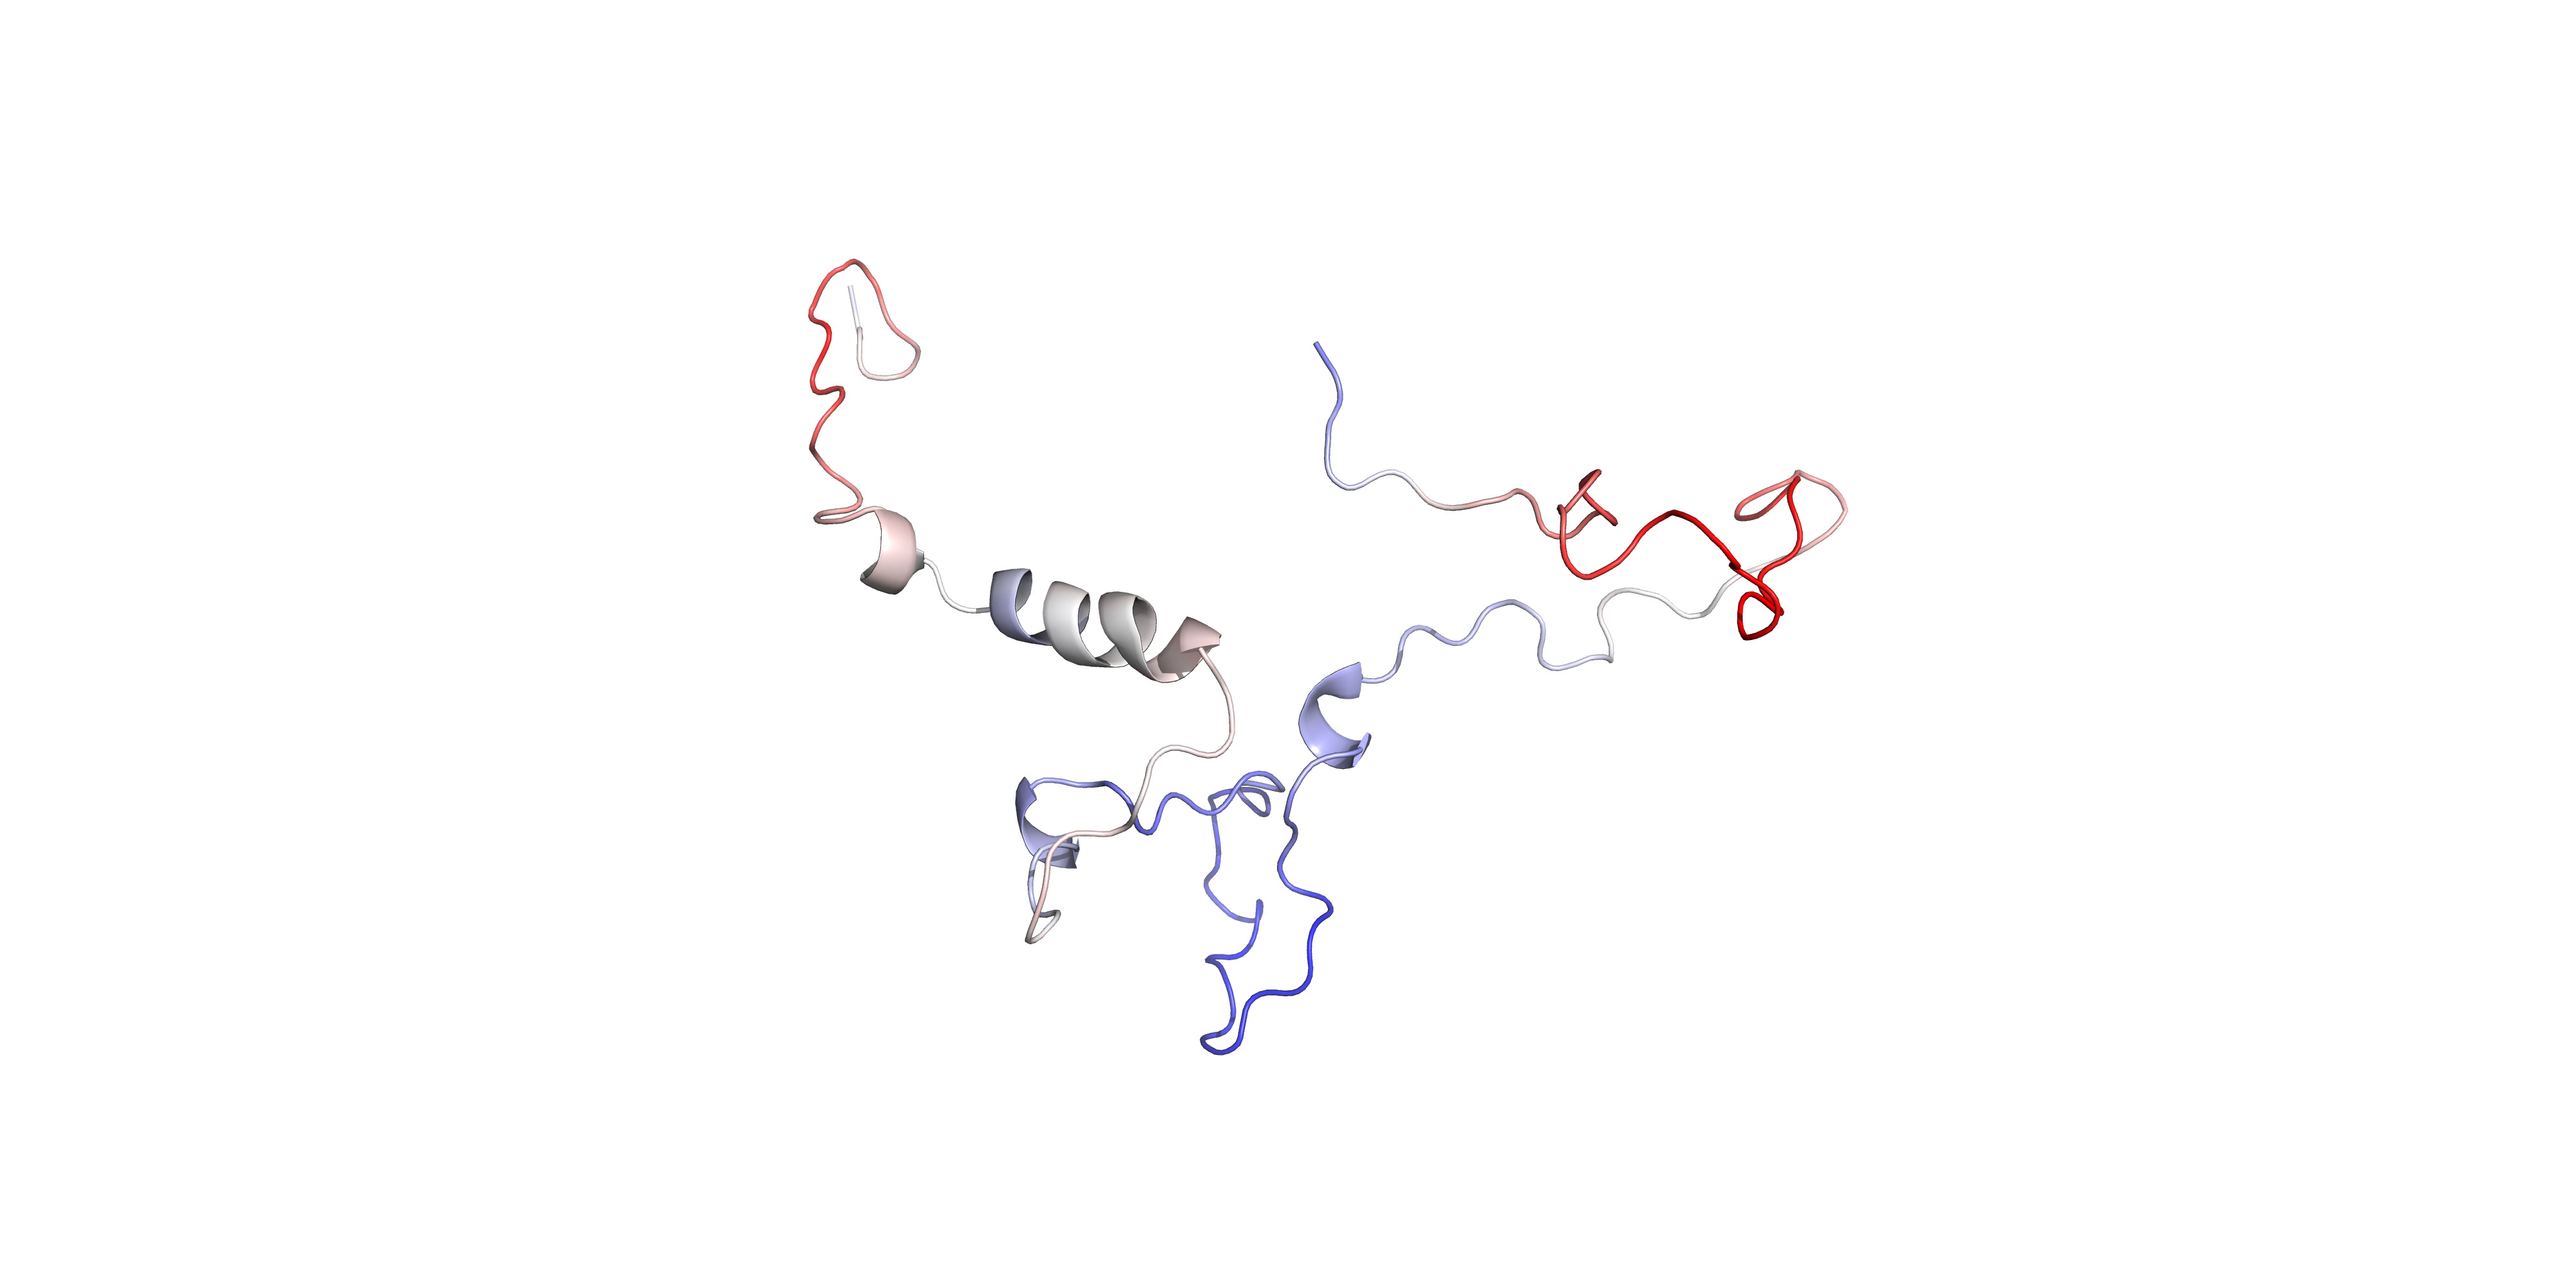
\includegraphics[width=\textwidth]{PED00020e004_pymol.png}
		\caption{Pymol image of ensemble 004 (model 118).}
		\label{model004p}
\end{figure}

\begin{figure}[H]
    \centering
		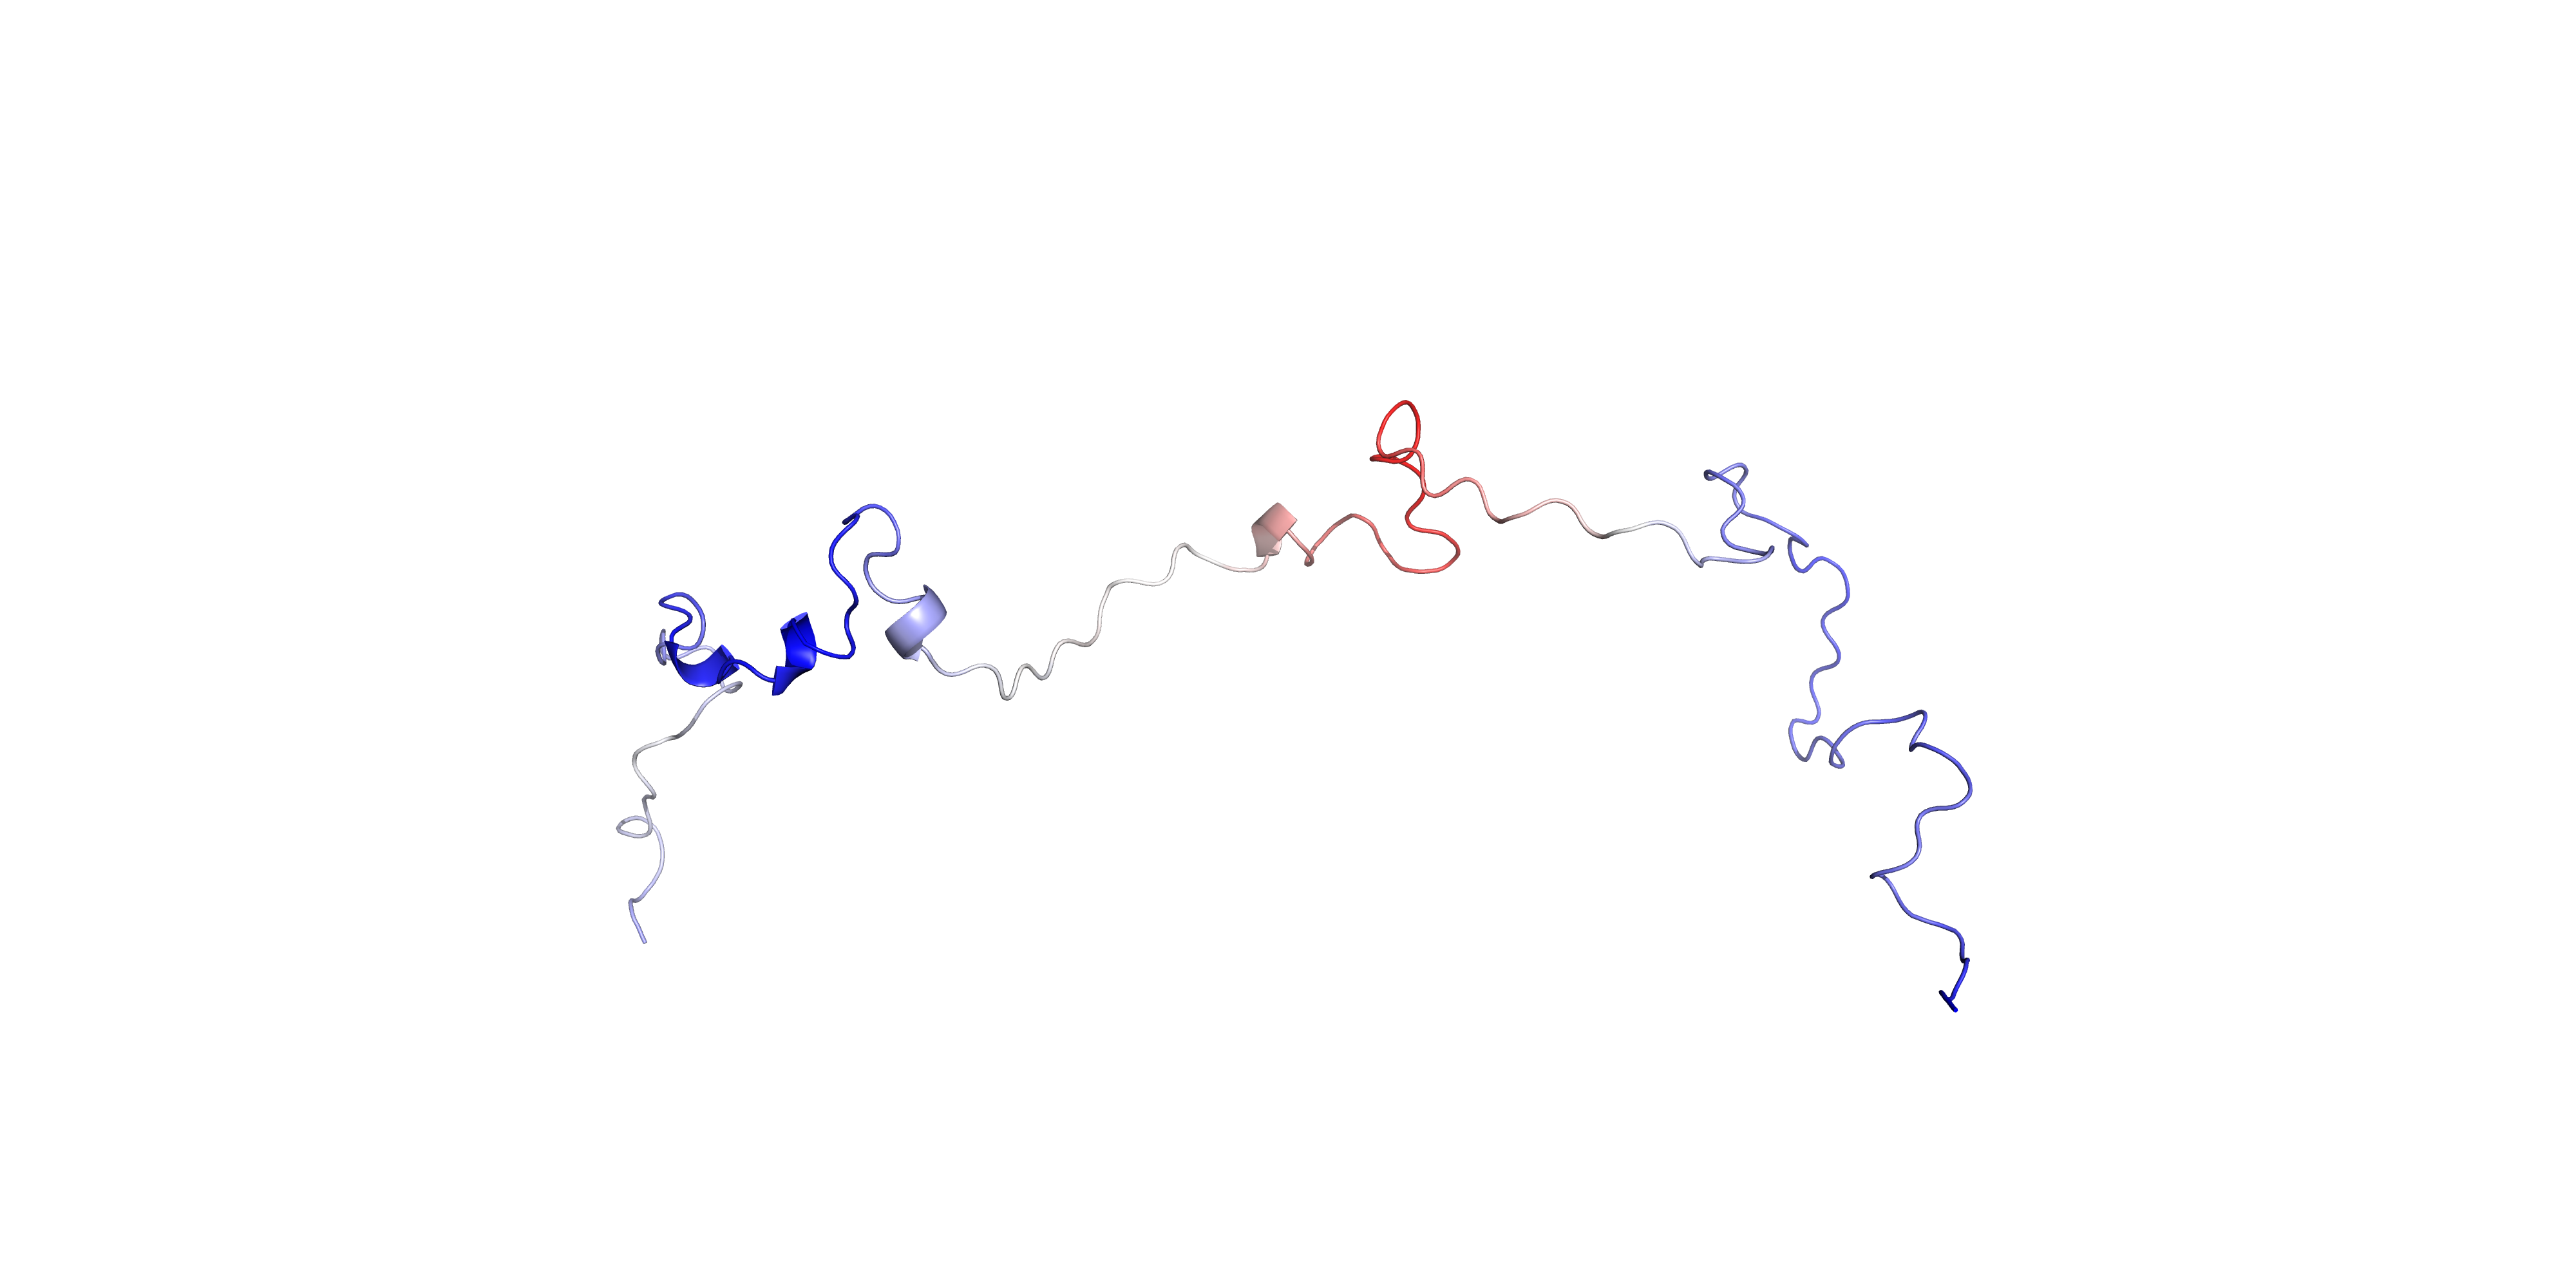
\includegraphics[width=\textwidth]{PED00020e005_pymol.png}
		\caption{Pymol image of ensemble 005 (model 133).}
		\label{model005p}
\end{figure}
